\begin{figure}[!ht]
    \centering
    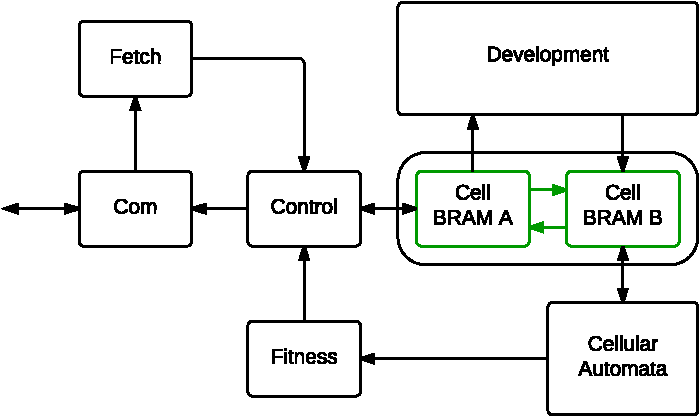
\includegraphics[width=0.8\textwidth]{implementation-simple}
    \caption{High-level block diagram of the new hardware platform.}
    \label{fig:implementation-simple}
\end{figure}

\begin{sidewaysfigure}[!pt]
    \centering
    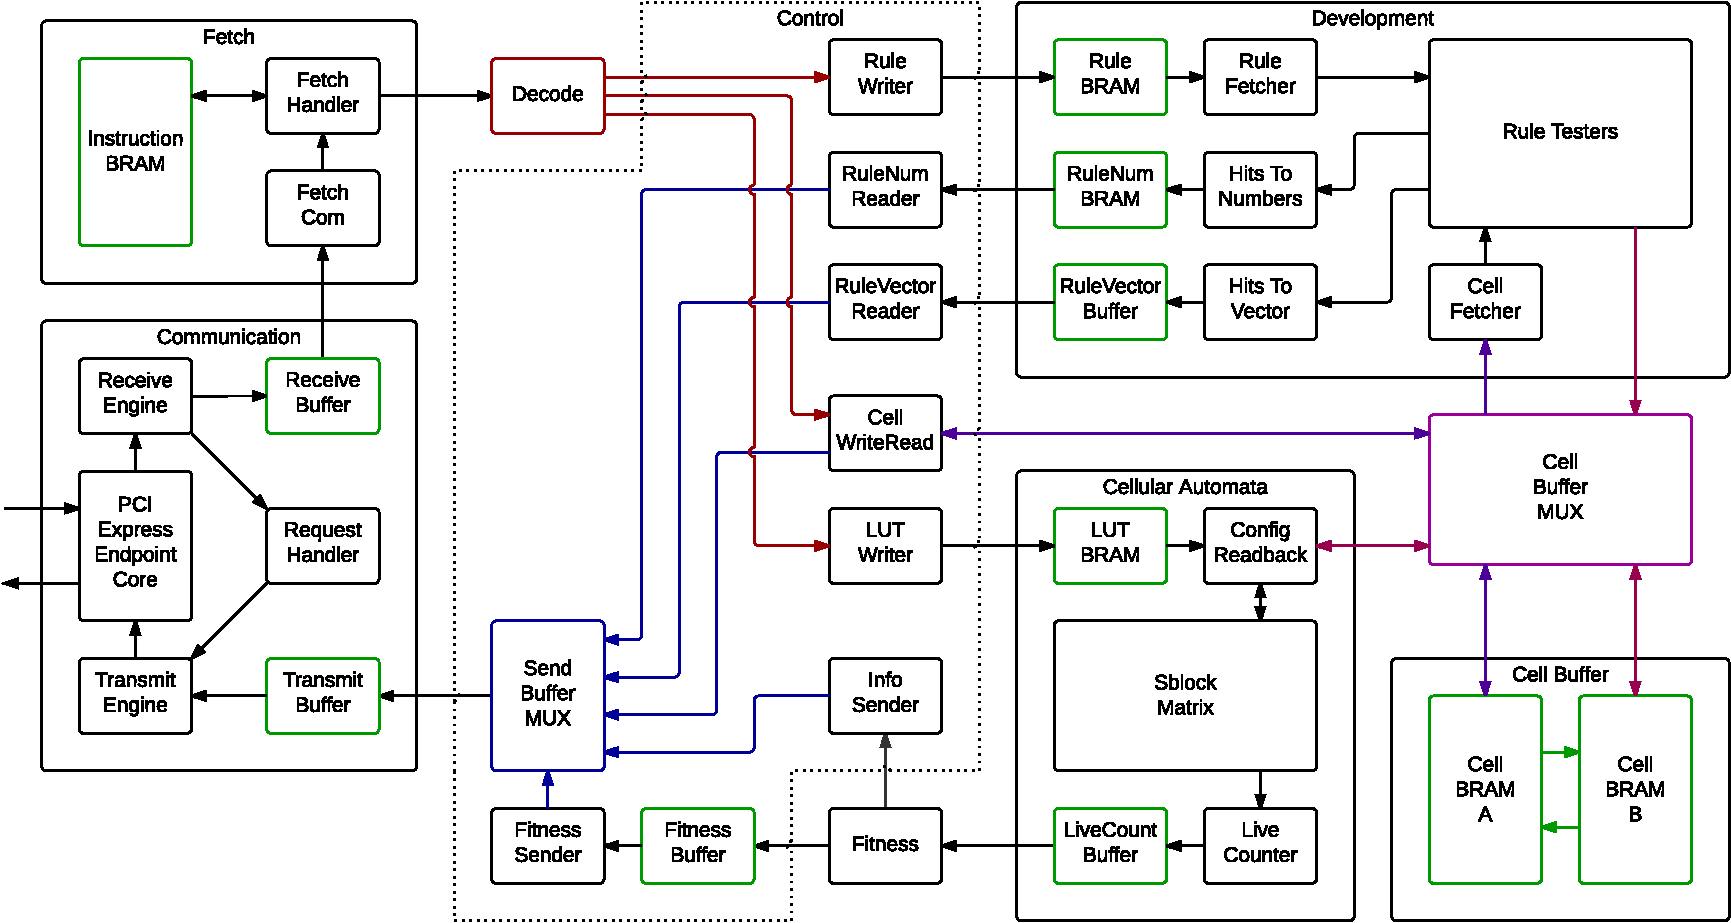
\includegraphics[width=\textwidth]{implementation-full}
    \caption[Detailed block diagram of the new hardware platform.]{
        Detailed block diagram of the new hardware platform.
        Control is implemented as a group of modules, marked by a dotted border.
        Some signals are color-coded for increased readability.
        Signals from Decode are colored red, while those to the Send and Cell Buffer Multiplexers are colored blue and purple respectively.
        Note the two different hues of purple for the different Cell BRAMs.
        Control signals are not shown.
    }
    \label{fig:implementation-full}
\end{sidewaysfigure}

The platform is design as an interlocked pipeline.
The main stages are Fetch, Decode and Execute, but due to interlocking, each stage can contain sub-pipelines or state machines.

The Execute stage is special in that is is split into many sub-modules, where only one is activated at a time.
The exception is Fitness, which is always active, since it operates in a dataflow-like fashion.
A hazard detection unit could be implemented to increase performance by allowing multiple non-conflicting units run in parallell.

Interlocking is implmented using special Run and Done signals.
Run is asserted when all modules asserts Done.

All state machines are of Mealy design with clocked output, unless noted otherwise.

\section{General Concepts}

\todo{Control signals not shown, only data}

\todo{Interlocking: run and done signals (need wavediagram)}

\todo{Timing / data passing between pipeline stages}

\todo{Borders: Green = BRAM, grey = outside}

\section{Communication}

The new communication unit is based on Xilinx' reference PCI Express programmed input/output design.
It consists of the Xilinx PCI Express endpoint core, reception and transmission engines, data buffers, and a special request handler, as shown in \figurename~\ref{fig:implementation-communication}.

\begin{figure}[!ht]
    \centering
    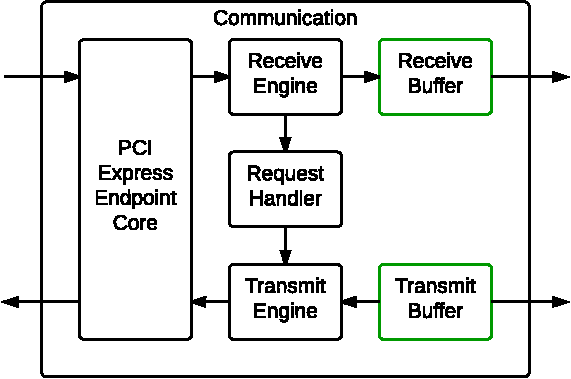
\includegraphics[width=0.7\textwidth]{implementation-communication}
    \caption[Communication module]{
        Detailed block diagram of the communication module.
    }
    \label{fig:implementation-communication}
\end{figure}

The endpoint core completely handles the physical and data link layers, and all TLPs related to configuration and establishment of the PCI Express connection.
Other TLPs, such as read and write requests, are presented on an AXI4-Stream interface \cite{ug672}.
The reception engine is responsible for parsing TLPs and either writing received data to the reception buffer or notifying the transmission engine about a read request.
The transmission engine is responsible for building completer TLPs to respond to read requests, using data from the transmission buffer.
The request handler listens to the read requests provided by the reception engine, and can override the transmission engine to respond to special requests.

\subsection{PCI Express Endpoint Core}

Several Spartan-6 FPGAs, including the one used in this project, contain a special-purpose hardware block for implementation of PCI Express.
The block completely handles the physical and data link layers, with the transaction layer left for the user.

To make use of the block, Xilinx provides the Spartan-6 Integrated PCI Express Endpoint Core; version 2.3 was used in this project.
This core additionally takes care of all TLPs related to configuration of the PCI Express connection.
Other TLPs, such as read and write requests, are presented on an AXI4-Stream interface \cite{ug672}.

The endpoint core is configured with two memory regions, both 4 kB in size\footnotemark.
\footnotetext{
    The smallest memory region that can be memory-mapped is one page. The default page size in Linux is 4 kB.
}
The first memory region (BAR0) is used for normal communication, while the second (BAR1) is used for special requests.
The separation is mostly conseptual as both regions are treated as one data stream.
The difference is that the special request handler kicks in for read requests to BAR1.

\subsection{Reception engine}

The reception engine is implemented as a simple state machine, as shown in \figurename~\ref{fig:statemachine-receive}.

\begin{figure}[!ht]
    \centering
    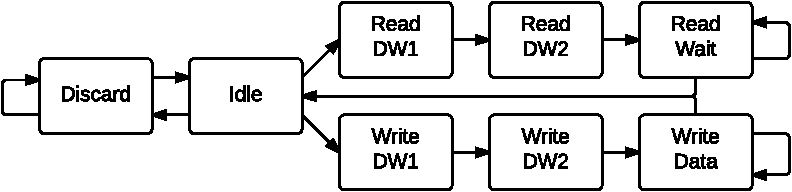
\includegraphics[width=0.8\textwidth]{statemachine-receive}
    \caption[Reception engine state machine]{
        State machine for the reception engine.
    }
    \label{fig:statemachine-receive}
\end{figure}

Until the endpoint core presents valid data, the state machine remains in Idle.
When it does, the data is stored, and the TLP type is checked.
If it is a read or write request, the state machine continues down the corresponding path, otherwise the remaining data is discarded.
The remaining portion of the TLP headers are then parsed in the DW1 and DW2 states.
For read requests, the state machine waits in ReadWait until the transmission engine is ready to accept a new read request, and then proceeds to Idle.
For write requests, the state machine stays in WriteData, where one DW of data is written to the reception buffer each cycle, for the length of the packet, and then proceeds to Idle.

\subsection{Transmission engine}

The transmission engine is implemented as a simple state machine, as shown in \figurename~\ref{fig:statemachine-transmit}.

\begin{figure}[!ht]
    \centering
    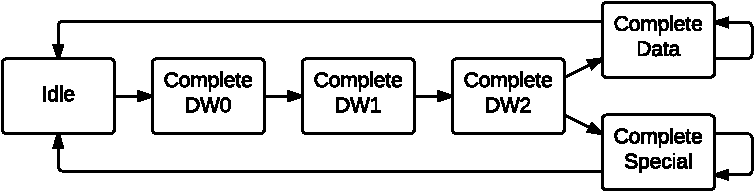
\includegraphics[width=0.8\textwidth]{statemachine-transmit}
    \caption[Transmission engine state machine]{
        State machine for the transmission engine.
    }
    \label{fig:statemachine-transmit}
\end{figure}

Until the reception engine signals a read request, the state machine remains in Idle.
When a read request is signaled by the reception engine, the state machine begins to traverse the DW path.
The DW0, DW1 and DW2 states each transmit one DW of the completer TLP header.
Then if the special request signal is set, it procceds to CompleteSpecial, where it transmits data presented by the request handler.
Otherwise, it proceeds to CompleteData where it transmits one DW of data from the transmission buffer each cycle.
When the requested number of DWs has been transmitted it proceeds back to Idle.

\subsection{Request handler}

The request handler continually listens to the read requests presented by the reception engine.
If the request is targeting the primary memory area (BAR 0), it is a normal read request and the transmission engine is allowed to proceed as usual.
Otherwise, it is a special request and the transmission engine is overridden.

The kind of special request is determined by the address of the read request, and handled thereafter.
There are currently four special requests implemented, as shown in Table~\ref{tab:requests}.

\begin{table}[!ht]
    \renewcommand{\arraystretch}{1.3}
    \label{tab:requests}
    \centering
    \begin{tabular}{c|l}
        \bfseries Address & \bfseries Request \\
        \hline
        0x00 & Get transmission buffer data count \\
        0x01 & Get transmission buffer available space \\
        0x02 & Get reception buffer data count \\
        0x03 & Get reception buffer available space \\
    \end{tabular}
    \caption{Special requests.}
\end{table}

Note that each of the implemented special requests assumes a read request length of one DW.
If the request has a greater length, the returned data is simply repeated to fill the packet.

\subsection{Buffers}

The buffers are implemented as first-in first-out (FIFO) queues using block RAM (BRAM) and two counters.
The counters determine the addresses that are written to and read from, and are incremented when the write or read signals are asserted.
\figurename~\ref{fig:wavediagram-fifo} shows how the FIFO is used to buffer two words.

\begin{figure}[!ht]
    \centering
    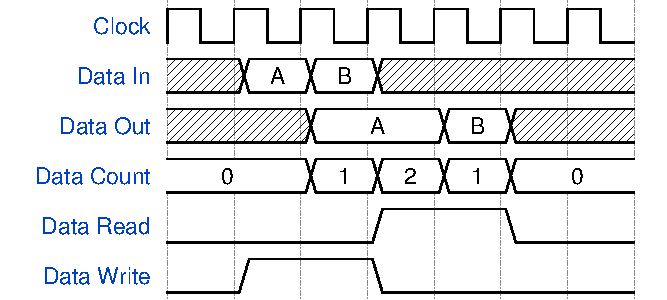
\includegraphics[width=0.7\textwidth]{figures/wavediagram-fifo}
    \caption[FIFO buffer wave diagram]{
        Wave diagram for the FIFO buffer, showing two consecutive writes followed by two consecutive reads.
    }
    \label{fig:wavediagram-fifo}
\end{figure}

Notice how the read signal needs to be asserted before the clock tick when data is read to ensure correct consecutive reads.
This is due to the BRAM used in the FIFO, which updates at clock ticks.
To have correct data available for a read in the following cycle, the address therefore has to be updated before the clock tick (by asserting the read signal).

\subsection{Software API}

The communication part of the new software API is split into two parts.

The first is a general interface for connecting to PCI and PCI Express devices without using a custom driver.
It takes advantage of Linux' automatic population of /sys/devices/pci* with files representing the memory regions of all PCI and PCI Express devices.
The directory is searched by vendor and device id, and the corresponding memory regions is memory-mapped into the program.

The second is an interface specifically for the communication unit.
It provides open, close, read and write functions similar to the old BenERA interface, in addition to implementing all special request functions in Table~\ref{tab:requests}.
When a read or write operation is initiated, buffers are checked for available data or space.
If there is not enough present, the program waits and then rechecks.

\section{Fetch}

Fetch is responsible for fetching the next instruction from either communication or internal memory.
It is also responsible for handling all control flow.

\begin{figure}[!ht]
    \centering
    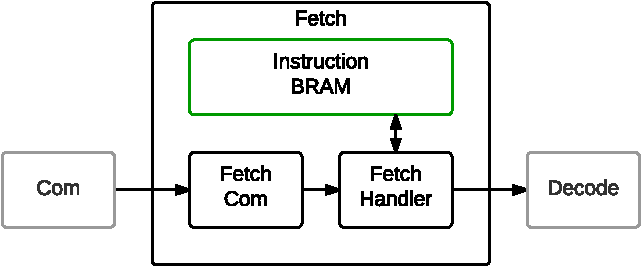
\includegraphics[width=0.7\textwidth]{implementation-fetch}
    \caption[Fetch module]{Detailed block diagram of the Fetch module.}
    \label{fig:implementation-fetch}
\end{figure}

\begin{figure}[!ht]
    \centering
    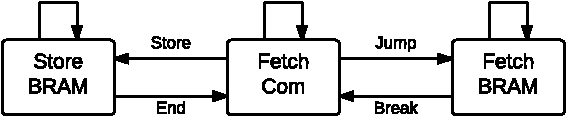
\includegraphics[width=0.6\textwidth]{statemachine-fetch-handler}
    \caption[Fetch Handler state machine]{State machine for the Fetch Handler.}
    \label{fig:statemachine-fetch-handler}
\end{figure}

It has three modes of operation: FetchCom, FetchMem and StoreMem.

In FetchCom mode, instructions are fetched from communication and sent to decode.
Since a variable-length format is used, this may take multiple cycles.
To make sure that instructions in the pipeline completes, NOPs are sent when the receive buffer is empty.
When encountering a Store instruction, it enters StoreMem mode and for a Jump instructions it enters FetchMem mode.

In FetchMem mode, instructions are fetched from InstructionBRAM and sent to decode.
The first InstructionBRAM address is specified by the Jump instruction, and then it is incremented by one after each instruction.
When encountering a Break instruction, it enters FetchCom mode.

In StoreMem mode, instructions are fetched from communication and stored in InstructionBRAM.
The first InstructionBRAM address is specified by the Store instruction, and then it is incremented by one after each instruction.
Instructions are stored in full 256-bit format.
When encountering an End instruction, it enters FetchCom mode.

Control flow is implemented by having N M-bit general counters and a JumpEqual instruction.
The counters can be incremented or reset using special instructions.
The JumpEqual instruction is treated as a Jump instruction when the specified counter matches the specified value, otherwise it is discarded.

\section{Decode}

Decode is responsible for parsing instructions, setting control signals and passing instruction parameters to activated modules.

The control signals determine which module is activated, which modules the CellBufferMux and SendBufferMux will connect to, and if the CellBuffer should swap contents.

%\section{RuleWriter}

%RuleWriter is responsible for writing development rules to RuleBRAM.

%The instruction parameter is simply stored to the BRAM.

%\section{RuleNumberReader}

%RuleNumberReader is responsible for transferring rule numbers from the RuleNumberBRAM to the SendBuffer.

%As many rule numbers as can fit 32 bits are sent each cycle, but it is aligned for each row.

%\section{LUTWriter}

%LUTWriter is responsible for writing a LUT entry to LUTBRAM.

%The instruction parameter is simply stored to the BRAM.

\section{Control}

\begin{itemize}
    \item Most very basic, but Cell Writer Reader very complex
    \item Rule Writer, LUT Writer pretty much the same
    \item Rule Number Reader similar to parts of Cell Writer Reader
    \item Fitness Sender
    \item Info Sender
\end{itemize}

\subsection{Cell Writer Reader}

\begin{itemize}
    \item Equivalent for Types
    \item Output is cropped and zero-extended
    \item Controlled by state machine
\end{itemize}

\begin{figure}[!ht]
    \centering
    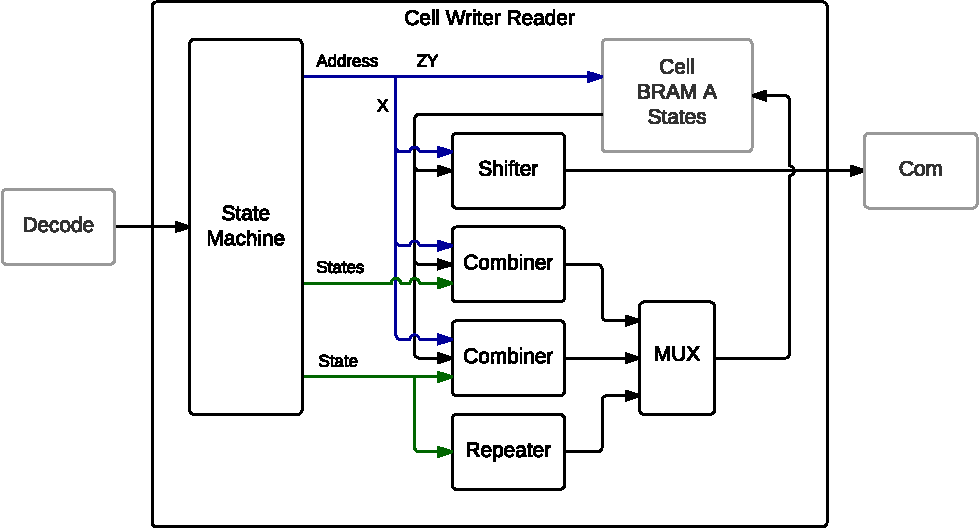
\includegraphics[width=\textwidth]{implementation-cell-writer-reader}
    \caption[Cell Writer Reader]{
        Detailed block diagram of the Cell Writer Reader.
        Only the state part is shown as the type part is identical.
        Cell BRAM A is drawn inside the module for completeness.
        Control signals are not shown.
    }
    \label{fig:implementation-cell-writer-reader}
\end{figure}

\begin{figure}[!ht]
    \centering
    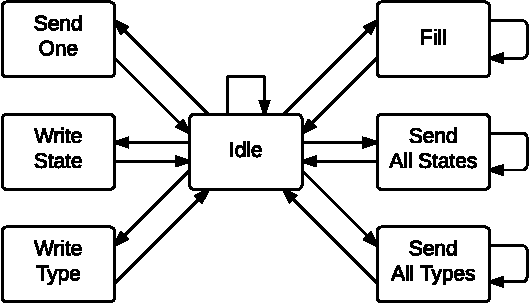
\includegraphics[width=0.55\textwidth]{statemachine-cell-writer-reader}
    \caption{Cell Writer Reader state machine}
    \label{fig:statemachine-cell-writer-reader}
\end{figure}

\section{Development}

Development is responsible for reading the cells in cell BRAM A, change them based on development rules specified by the user, and write the result to cell BRAM B.

It is implemented as a state machine controlling an interlocked two-stage pipeline.

The first stage is CellFetch, which reads the cell neighborhoods for one row of cells per run.
\todo{explain access pattern}
This takes 3 cycles for 2D and 5 for 3D.

The second stage is implemented as yet another pipeline.
First, rules are fetched from RuleBRAM, then rules and cell neighborhoods are sent to the RuleTesters.
To allow multiple rules to be tested each cycle, RuleTesters is split into two parts.
The first part tests the different rules against each cell, while the second selects the result from the highest priority rule.
After the first part, hits are output from RuleTesters to HitsToVector and HitsToNumbers.
Finally, everything is stored to memory.
\footnote{Rule vectors are only stored after the final rules and cells}

The number of active rules can be set at runtime to reduce development time by skipping unused rules.
\TODO
\todo{CellFetch limiting factor for very few rules}
\todo{vectors overwritten to allow development without reading them}

\begin{itemize}
    \item Rule 0 reserved.
    \item Two-stag pipeline:
    \begin{itemize}
        \item CellFetch
        \item RuleFetch, Test, HitsToVec/Num, Write (4-stage pipeline)
    \end{itemize}
    \item Last triggered rules are written to RuleNumbersBRAM
    \item All triggered rules are written to RuleVectorBuffer (even overridden)
\end{itemize}

\begin{figure}[!ht]
    \centering
    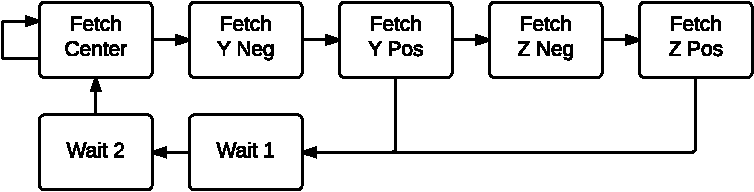
\includegraphics[width=0.8\textwidth]{statemachine-cell-fetcher}
    \caption[Cell Fetcher state machine]{
        State machine for the Cell Fetcher.
    }
    \label{fig:implementation-cell-fetcher}
\end{figure}

\begin{figure}[!ht]
    \centering
    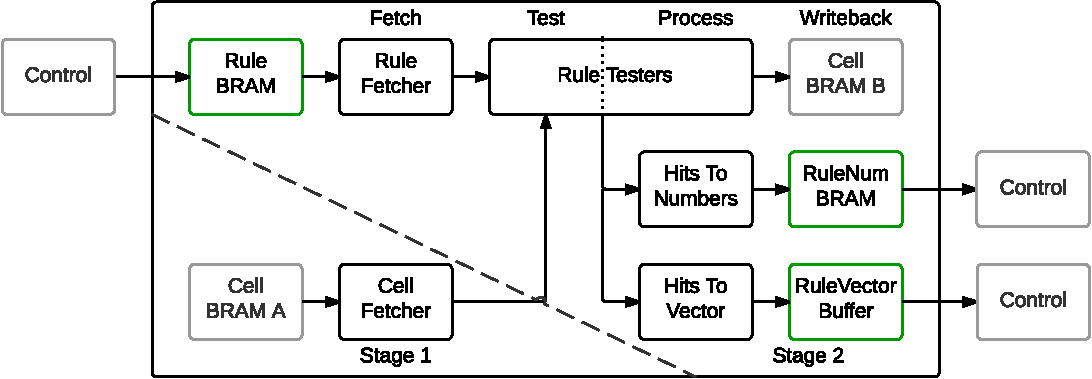
\includegraphics[width=\textwidth]{implementation-development}
    \caption[Development module]{
        Detailed block diagram of the Development module.
        The two main pipeline stages are separated by a dashed line,
        while the substages of the pipeline within the second main stage are marked at the top.
        The cell BRAMs are drawn inside the module for pipeline completeness.
        Control signals are not shown.
    }
    \label{fig:implementation-development}
\end{figure}

\begin{figure}[!ht]
    \centering
    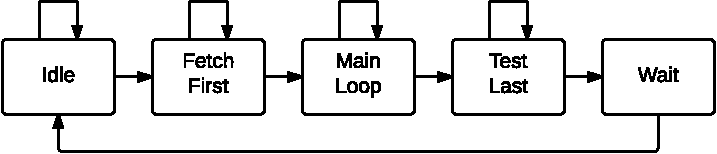
\includegraphics[width=0.75\textwidth]{statemachine-development}
    \caption[Development module state machine]{
        State machine controlling the Development module.
    }
    \label{fig:statemachine-development}
\end{figure}

\section{Cellular Automata}

The Cellular Automata module is responsible for configuring the sblock matrix with data from the Cell Buffer, step the sblocks and store the number of live cells, and read the new states back into the Cell Buffer.

It is implemented as a state machine that is manipulating a matrix of sblocks connected to an adder tree.
The adder tree is used to calculate the number of live cells after each step.
The numbers are then stored in the Live Count Buffer.
If the Live Count Buffer is full, data is overwritten, possibly corrupting fitness evaluation, until the buffers are reset.
This design decision was made to allow the CA to run without being required to read fitness data.

When configuring the sblock matrix, cell types are used as an index for the LUTBRAM to find the corresponding LUT entry.

\begin{figure}[!ht]
    \centering
    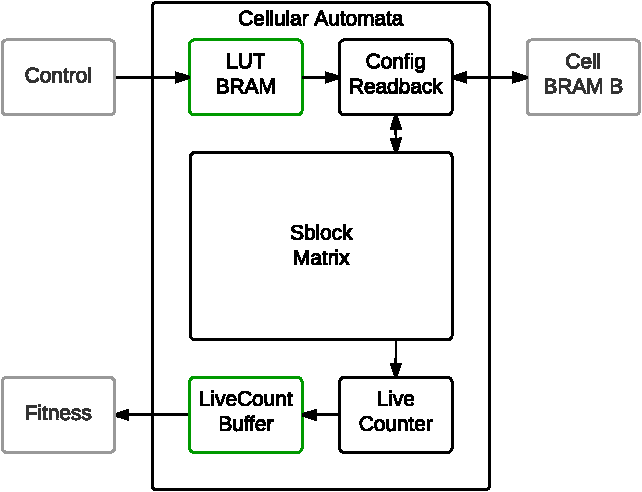
\includegraphics[width=0.7\textwidth]{implementation-cellular-automata}
    \caption[Cellular Automata]{
        Detailed block diagram of the Cellular Automata.
    }
    \label{fig:implementation-cellular-automata}
\end{figure}

\begin{figure}[!ht]
    \centering
    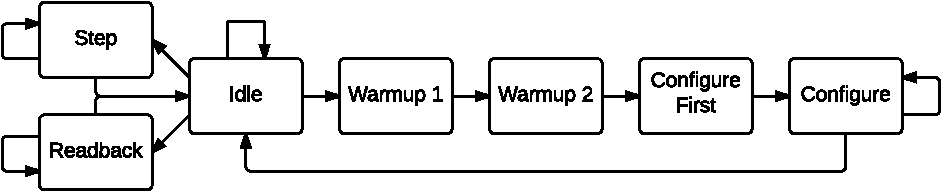
\includegraphics[width=\textwidth]{statemachine-cellular-automata}
    \caption[Cellular Automata state machine]{
        State machine controlling the Cellular Automata.
    }
    \label{fig:statemachine-cellular-automata}
\end{figure}

\begin{itemize}
    \item ConfigReadback is not separate module, but statemachine in CA
\end{itemize}

\section{Fitness}

\begin{itemize}
    \item Dataflow-ish (livecountbuffer to fitnessbuffer)
    \item Custom implementation, simple interface
\end{itemize}

\subsection{Live Count}

\todo{simply copies from Live Count Buffer to Fitness Buffer}

\subsection{Discrete Fourier Transform}

\begin{itemize}
    \item Revised version of Ola Martin's
    \item More customizable (describe parameters)
    \item Copies Data to internal buffer, since FIFO is delete-on-read (fig)
\end{itemize}

\todo{where? also tweak language}
By default, neighbors which would be outside the matrix are treated as having a state and type of zero.
However, when matrix wrap is enabled, neighbors on the opposite side of the matrix are used instead.
This applies to both runstep and devstep.
